\setcounter{chapter}{0}
\chapter{Introduction} \label{chap::introduction}
This template is designed to define the thesis format for Pablo de Olavide University (\acs{UPO}). It showcases LaTeX’s capabilities in creating professional-looking documents, including examples of tables, figures, mathematical formulas, floating content, and citations. All content is provided as placeholder text to illustrate how to format and structure your own document.

\section{Section example} \label{sec::section_example}
\subsection{Complex Tables}

In this section \ref{sec::section_example}, we provide an example of a complex table with multiple columns and rows, such as a table of results.

\begin{table}[htbp]
    \centering
    \caption{Results of Experiments}
    \begin{tabular}{@{}cccccc@{}}
        \toprule
        \textbf{Experiment} & \textbf{Parameter A} & \textbf{Parameter B} & \textbf{Result 1} & \textbf{Result 2} & \textbf{Conclusion} \\ 
        \midrule
        Exp 1 & 10 & 5 & 0.95 & 0.88 & Pass \\
        Exp 2 & 15 & 7 & 0.92 & 0.87 & Fail \\
        Exp 3 & 20 & 9 & 0.89 & 0.85 & Pass \\
        Exp 4 & 25 & 10 & 0.85 & 0.80 & Pass \\
        \bottomrule
    \end{tabular}
\end{table}

This table shows how to include multiple columns and rows, using the `booktabs` package for clearer lines between rows.

\subsection{Floating Figures and Skipping Content}

When figures are placed within a document, they often float to an optimal location. Below is an example of a figure that may float and break the content flow. This is useful in cases where strict figure placement is not necessary.

\begin{figure}[htbp]
    \centering
    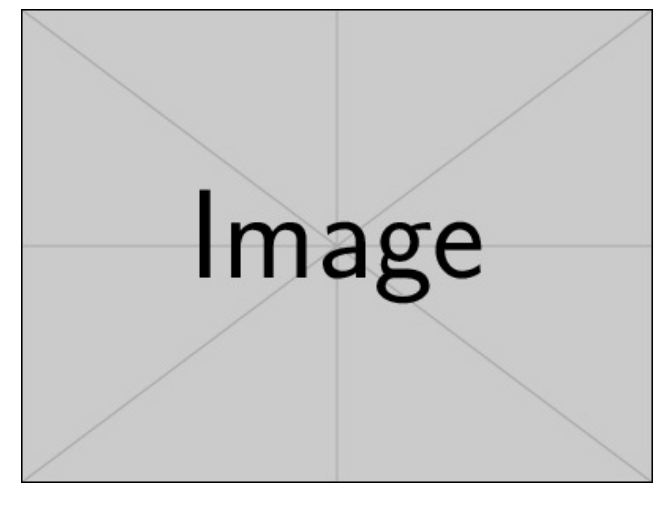
\includegraphics[width=0.5\textwidth]{figures/sample_image.png}
    \caption{A floating figure that may move to an optimal position in the document.}
    \label{fig::floating_figure}
\end{figure}

\begin{color}{gray}
  \lipsum[1]  % Placeholder text to show how figures float
  \lipsum[2]	contenidos...
\end{color}


\subsection{Figures with Black Boxes and Captions}

The following is an example of how to insert a figure with a black box around it, including a caption.

\begin{figure}[H]
    \centering
    \fbox{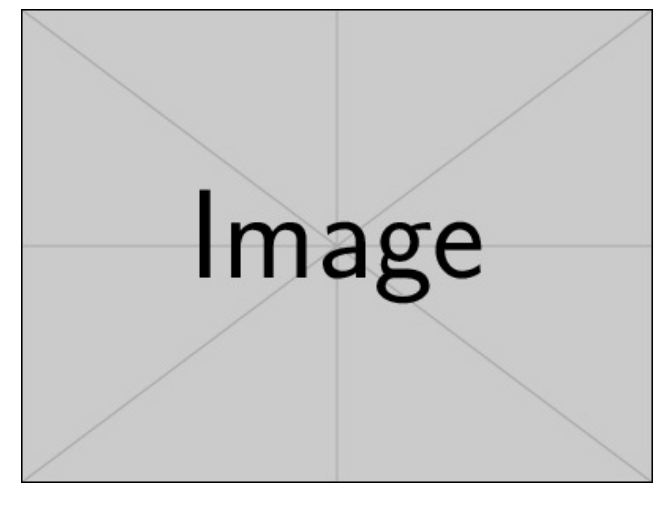
\includegraphics[width=0.6\textwidth]{figures/sample_image.png}}
    \caption{This is a sample figure inside a black box. Captions should be informative and concise.}
    \label{fig::sample_figure}
\end{figure}

This figure uses the `fbox` command to place a black border around the image, and the `caption` package allows you to customize the figure's caption.


\subsection{Wrapping Text Around Figures}

You can also wrap text around a figure, which is helpful when you want to integrate an image into your text without breaking the flow.

\begin{wrapfigure}{R}{0.4\textwidth}
    \centering
    \fbox{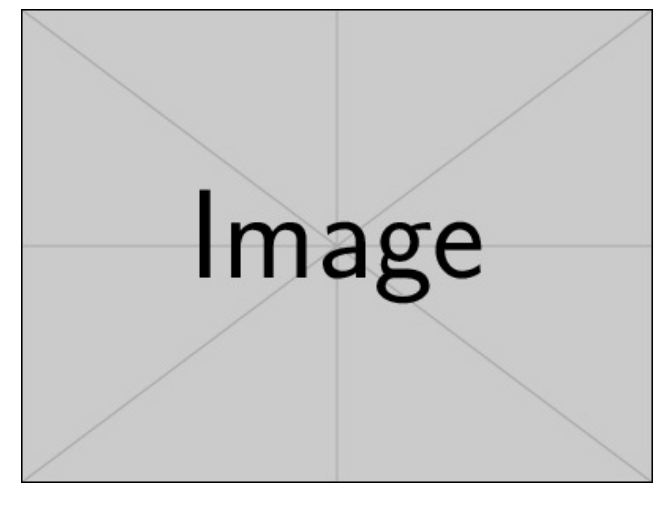
\includegraphics[width=0.38\textwidth]{figures/sample_image.png}}
    \caption{Text wrapped around this figure.}
    \label{fig::wrap_figure}
\end{wrapfigure}

\begin{color}{gray}
  \lipsum[4-6]
\end{color}

The `wrapfig` package allows text to flow around figures, which can enhance the layout of your document when integrating images, as in the figure \ref{fig::wrap_figure}.

\subsection{Mathematical Formulas}

Mathematical expressions can be written in both inline and display style. Here are some examples:

Inline formula: $E = mc^2$.

Display-style formula:

\[
\sum_{i=1}^n i = \frac{n(n+1)}{2}
\]

A more complex equation involving integrals:

\[
\int_{0}^{\infty} e^{-x^2} \, dx = \frac{\sqrt{\pi}}{2}
\]

\subsection{List Structures}

LaTeX supports various types of lists, including unordered, ordered, and description lists.
Unordered list:
\begin{itemize}
    \item First item
    \item Second item
    \item Third item
\end{itemize}
List with bullet point changed:
\renewcommand\labelitemi{\ding{117}}
\begin{itemize}
	\item First item
	\item Second item
	\item Third item
\end{itemize}
Ordered list:
\begin{enumerate}
    \item Step 1
    \item Step 2
    \item Step 3
\end{enumerate}
Description list:
\begin{description}
    \item[Term 1] Definition of the first term.
    \item[Term 2] Definition of the second term.
\end{description}

\subsection{Citations and References}

In academic writing, citations are crucial. Below is an example of a citation using a bibliography entry.

You can cite references in the text like this: \cite{fakeauthor2022article}, \cite{fakeauthor2021book}, \cite{fakeauthor2020conference}, \cite{fakeauthor2019report}, \cite{fakeauthor2018thesis}, \cite{fakeauthor2021website}, \cite{fakeauthor2022github}, \cite{fakeauthor2017chapter}, \cite{fakeauthor2023workshop}, \cite{fakeauthor2020manual}.

\begin{paragraph}{Run-in Heading:}
This is an example of a paragraph with a table on it:
\begin{table}[htbp]
	\begin{center} {\footnotesize
			\begin{tabularx}{\textwidth}{@{} lXlX @{} }
				\multicolumn{2}{c}{} \\ 
				\hline
				
				\normalsize \textbf{Category} & \normalsize \textbf{Description} \\
				
				\hline
				& \\
				Example 1 & Lorem ipsum dolor sit amet, consectetur adipiscing elit. Phasellus bibendum est ut lacus bibendum, non fermentum ex ultricies. Praesent id ipsum sed elit ultricies facilisis. Fusce posuere odio ac tortor gravida, a viverra nibh pretium. \\
				& \\
				Example 2 & Lorem ipsum dolor sit amet, consectetur adipiscing elit. Integer ac nisl eget nulla ultrices venenatis. Vestibulum ante ipsum primis in faucibus orci luctus et ultrices posuere cubilia curae. Donec euismod orci et turpis malesuada, in posuere nisl euismod. \\
				& \\
				Example 3 & Lorem ipsum dolor sit amet, consectetur adipiscing elit. Aliquam sed justo sit amet nisi interdum sodales. Nam eget augue eu sapien scelerisque tempor. Curabitur tincidunt turpis vitae dolor consectetur, ut accumsan erat feugiat. Vestibulum ante ipsum primis in faucibus orci luctus et ultrices posuere cubilia curae. \\
				\hline
		\end{tabularx}}
	\end{center}
	\caption{\footnotesize Example table multicolum}
	\label{tab::example_table_multicolumn}
\end{table}
\end{paragraph}

\subsection{Subsection with icon \icon{figures/sample_image.png}}
Finally, this is an example how to place an icon in a subsection title.

\section{What is LATEX?}
LATEX (pronounced "Lah-tech" or "Lay-tech") is a macro package created by Leslie Lamport based on TEX. As a document preparation system for high-quality typesetting in almost any forms of publishing, LATEX is not the name of a particular editing program, but refers to the encoding or tagging conventions that are used in LATEX documents.

\section{Why use LATEX?}
There are many good reasons to use LATEX. The most significant ones are:
\begin{itemize}
	\item It allows you to clearly separate the content from the format of your document.
	\item It lets you concentrate on your ideas, not the visual appearance.
\end{itemize}

\section{How to use?}
\subsection{Installation}
LaTeX is based on open-source code, so it is available on most platforms as free software. Depending on your operating system, you may encounter different installation instructions.

\begin{itemize}
	\item \textbf{Linux:} TeXLive distribution.
	\item \textbf{MacOS:} MacTeX or TeXLive.
	\item \textbf{Windows:} MiKTeX or TeXLive.
\end{itemize}

\section{How to write the introduction}
The introduction is a crucial section of any research paper, as it establishes the writing style, research quality, and credibility of the author. It provides readers with the necessary background and context to understand the importance of the research being presented. This section begins by broadly introducing the research topic and then narrows down to a specific research question or hypothesis. 

According to the San José State University Writing Center \cite{SJSUWritingCenterIntroduction}, the introduction serves to answer three fundamental questions: (1) What is the research about? (2) Why is it important? (3) What does the author want the reader to understand? 

A well-structured introduction starts with a general overview of the topic, supported by recent research, and gradually becomes more focused, leading to the specific research problem. The introduction should avoid going too in-depth, as detailed analyses are reserved for the body of the paper. Instead, it highlights the research focus, problem statement, and objectives, aligning with the standards of the discipline. Furthermore, it is essential to differentiate between the introduction and the literature review, as the latter critically evaluates existing research, while the introduction sets the stage for the study \cite{SJSUWritingCenterIntroduction}.

In various academic disciplines, the introduction may differ in tone, structure, and content. For instance, in business and engineering, clarity and conciseness are paramount, while in the humanities, there is more room for creativity in presenting the research problem \cite{SJSUWritingCenterIntroduction}. Regardless of the field, a well-crafted introduction should follow a clear organizational structure, often visualized as an inverted triangle, beginning with broad context and narrowing to specific research questions. 

The San José State University Writing Center recommends utilizing the Create a Research Space (CARS) model, which involves three steps: (1) establishing the relevance of the topic, (2) identifying gaps or limitations in existing research, and (3) filling those gaps with the research question, hypothesis, or objectives \cite{SJSUWritingCenterIntroduction}. By following this model, the introduction effectively conveys the significance of the research and guides the reader toward understanding its purpose and scope.
